\documentclass[a4paper]{article}
\usepackage[T1]{fontenc}
\usepackage[utf8]{inputenc}
% \usepackage[swedish]{babel}
\usepackage{fancyvrb}
\usepackage{graphicx}
\usepackage{biblatex}
\usepackage{verbatim}
\usepackage{listings}
\usepackage{xcolor}
\usepackage{url}
\usepackage{amsmath}

\addbibresource[]{assignment3.bib}
\fvset{tabsize=4}
\fvset{fontsize=\small}

\definecolor{codegreen}{rgb}{0,0.6,0}
\definecolor{codegray}{rgb}{0.5,0.5,0.5}
\definecolor{codepurple}{rgb}{0.58,0,0.82}
\definecolor{backcolour}{rgb}{0.95,0.95,0.92}
\lstdefinestyle{mystyle}{
    backgroundcolor=\color{backcolour},   
    commentstyle=\color{codegreen},
    keywordstyle=\color{magenta},
    numberstyle=\tiny\color{codegray},
    stringstyle=\color{codepurple},
    basicstyle=\footnotesize,
    breakatwhitespace=false,         
    breaklines=true,                 
    captionpos=b,                    
    keepspaces=true,                 
    numbers=none,                    
    numbersep=5pt,                  
    showspaces=false,                
    showstringspaces=false,
    showtabs=false,                  
    tabsize=2
}
\lstset{style=mystyle}

\title{TFRP20 Artificial Intelligence (VT25)\\ Assignment 3: Classification with the perceptron and logistic regression}
\author{Anders Holm\\\texttt{anders.holm@senspix.net} \and
Magnus Gäfvert\\\texttt{magnus.gafvert@gmail.com}}
\date{2025--03--10}
\begin{document}
\maketitle
\begin{abstract}
    This report present and discuss the authors' solution to an assignment on classification with the perceptron and logistic regression in teh Artificial Intelligence course given at the Department of Computer Science at Lund University in the spring of 2025. The solution is implemented in the given template Jupyter notebook and provided alongside this report.
\end{abstract}

\section{Introduction}
The objectives of this assignment~\cite{tfrp20assignment3} are to:

\begin{enumerate}
    \item  Write a linear regression program using gradient descent;
    \item  Write linear classifiers using the perceptron algorithm and logistic regression;
    \item  Experiment variations of the algorithms;
    \item  Evaluate classifiers;
    \item  Experiment with popular tools;
    \item  Read a scientific article on optimization techniques and comment it;
    \item  Present code, results, and comments in a short dissertation. 
\end{enumerate}

The respective tasks are presented in the following sections.

\section{Method}
The implementation toolchain is based on Jupyter Notebook with numpy with Python 3.9.21 and the Anaconda distribution~\cite{anaconda} using Microsoft Visual Studio Code with free GitHub Copilot served by the preview Anthropic Claude 3.5 Sonnet LLM and Microsoft Python plugins. This report is typeset with \LaTeX using TexLive and and the LaTeX Workshop plugin by James Yu.

The code is structured in a Jupyter notebook: 
\begin{verbatim}
    ai_lab_perceptron_students.ipynb    
\end{verbatim}
with sections and cells for each of the tasks in the assignment, and handed in together with this report. The code is evaluated with the provided evaluation data from the historial novel Salammbô by Gustave Flaubert~\cite{flaubert1862salammbô} in original French and in English translation to verify performance of the implementation.

 
\section{Results and discussion}


\subsection{Linear regression program using gradient descent}

Linear regression with gradient descent in batch and stochastic variants as described in \cite[pp. 694--697]{aima} are implemented based on~\cite{nugues_lectures_2025} in the Jupyter notebook. The algorithms are applied on the provided word and letter 'a' counts from the 15 chapters of~\cite{flaubert1862salammbô} in French and English. The result is shown in Figure~\ref{fig:regression_English_French} with final weights  summarized in Table~\ref{tab:regression-table}, and with convergence speeds illustrated in Figure~\ref{fig:regression_errors}. 
\begin{figure}
    \centering
    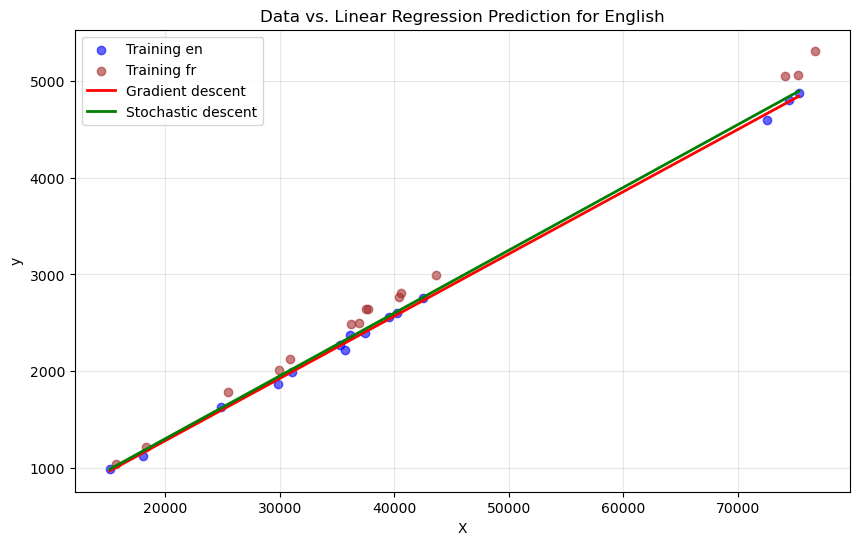
\includegraphics[width=0.45\textwidth]{figures/Fit English.png}
    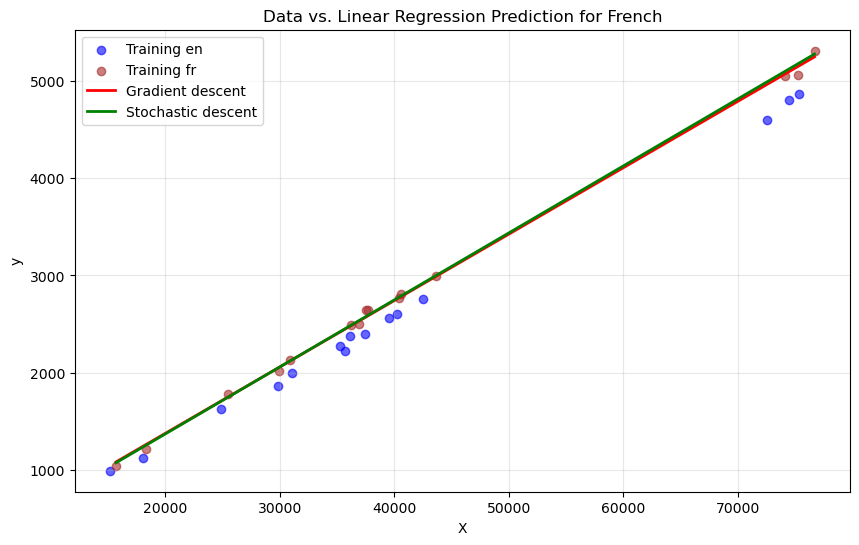
\includegraphics[width=0.45\textwidth]{figures/Fit French.png}
    \caption{Linear regression of letter 'a' and word counts with batch and gradient descent trained on English translation (left) and French original (right) of cite{flaubert1862salammbô}.}
    \label{fig:regression_English_French}
\end{figure}


\begin{figure}
    \centering
    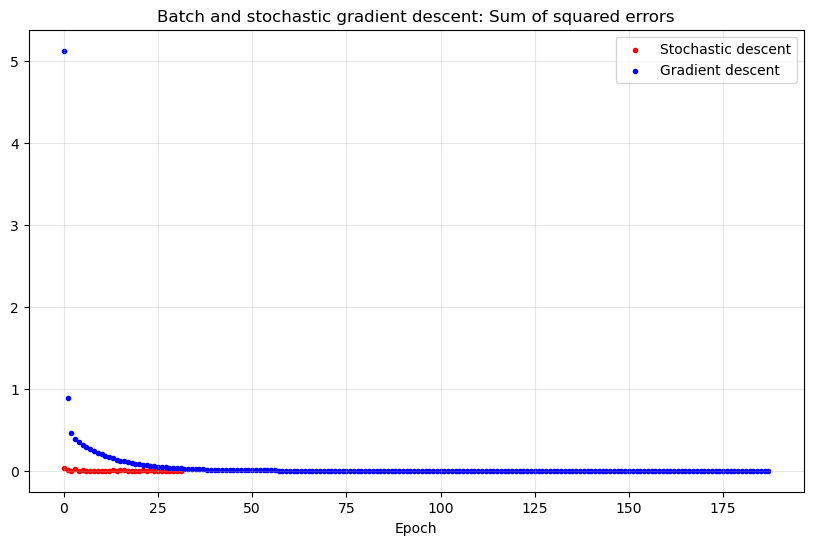
\includegraphics[width=0.8\textwidth]{figures/Regression errors.png}
    \caption{Comparison of onvergence of the batch and stochastic versions of linear regression trained on \cite{flaubert1862salammbô}.}
    \label{fig:regression_errors}
\end{figure}

\begin{table}[]
    \caption{Regression results}
    \label{tab:regression-table}
    \small
    \begin{tabular}{lllll}
        \hline\hline
             & \multicolumn{2}{c}{French}                    & \multicolumn{2}{c}{English}            \\
             & Gradient descent & Stochastic descent & Gradient descent & Stochastic descent \\
             \hline
    Epoch    & 187              & 31                 & 186              & 15                 \\
    w{[}0{]} & 0.00170945       & -0.00170833        & -6.71530774e-04  & 0.00111656         \\
    w{[}1{]} & 0.98640986       & 0.99526806         & 9.94590530e-01   & 1.00362464\\
    \hline
    \end{tabular}
\end{table}


\subsection{Linear classifiers using the perceptron algorithm and logistic regression}
The stochastic perceptron program with hard threshold as described in \cite[pp. 700--702]{aima} is implemented based on~\cite{nugues_lectures_2025} in the Jupyter notebook as suggested with \verb|fit(X,y)| and \verb|predict(X,w)| functions. The algorithms are applied on the provided word and letter 'a' counts from the 15 chapters of~\cite{flaubert1862salammbô} in French and English. The result is shown in Figure~\ref{fig:Stochastic_descent} (top) with successful separation of the data points for French and English. Leave-one-out cross-validation is shown in Figure~\ref{fig:classifier_result} (top), with 100\% success rate.

The stochastic logistic regression program as described in \cite[pp. 702--705]{aima} is likewise implemented based on~\cite{nugues_lectures_2025} in the Jupyter notebook. The algorithms are applied on the same data set. The result is shown in Figure~\ref{fig:Stochastic_descent_logistic_classifier} with successful separation of the data points for French and English. Leave-one-out cross-validation is shown in Figure~\ref{fig:classifier_result}, with 100\% success rate. The logistic surface is illustrated in Figure~\ref{fig:logistic_classifier}.

\begin{figure}
    \centering
    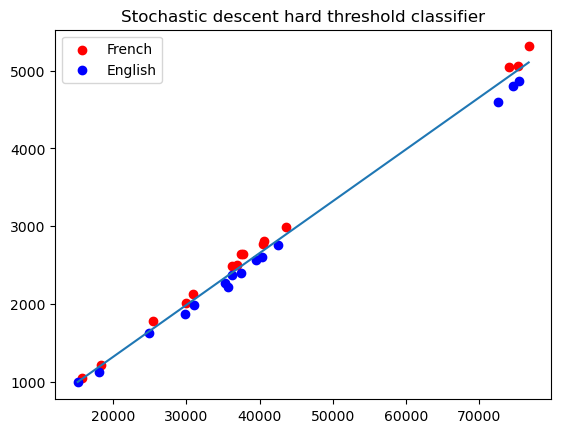
\includegraphics[width=0.45\textwidth]{figures/Stochastic descent hard threshold classifier.png}
    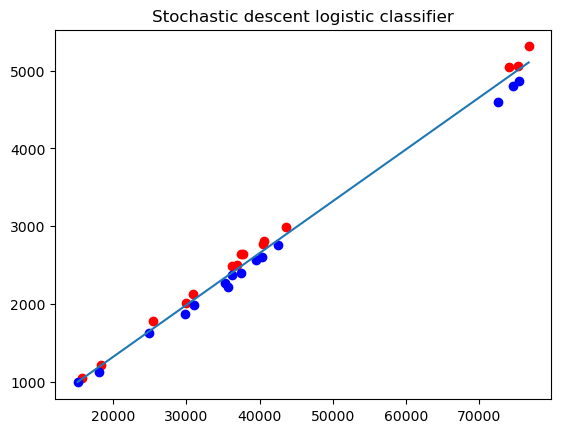
\includegraphics[width=0.45\textwidth]{figures/Stoschastic descent logistic classifier.png}
    \caption{Linear classifier with hard threshold (left) and logistic function (right).}
    \label{fig:Stochastic_descent}
\end{figure}


\begin{figure}
    \centering
    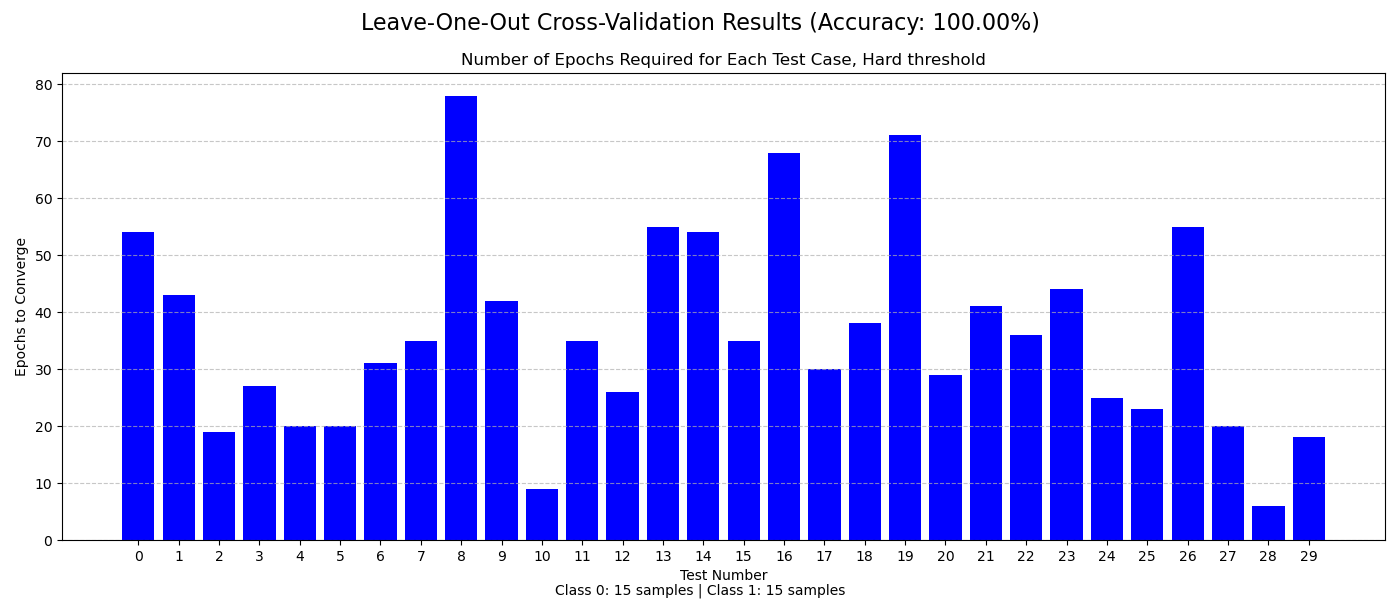
\includegraphics[width=0.8\textwidth]{figures/classifier result 1.png}
    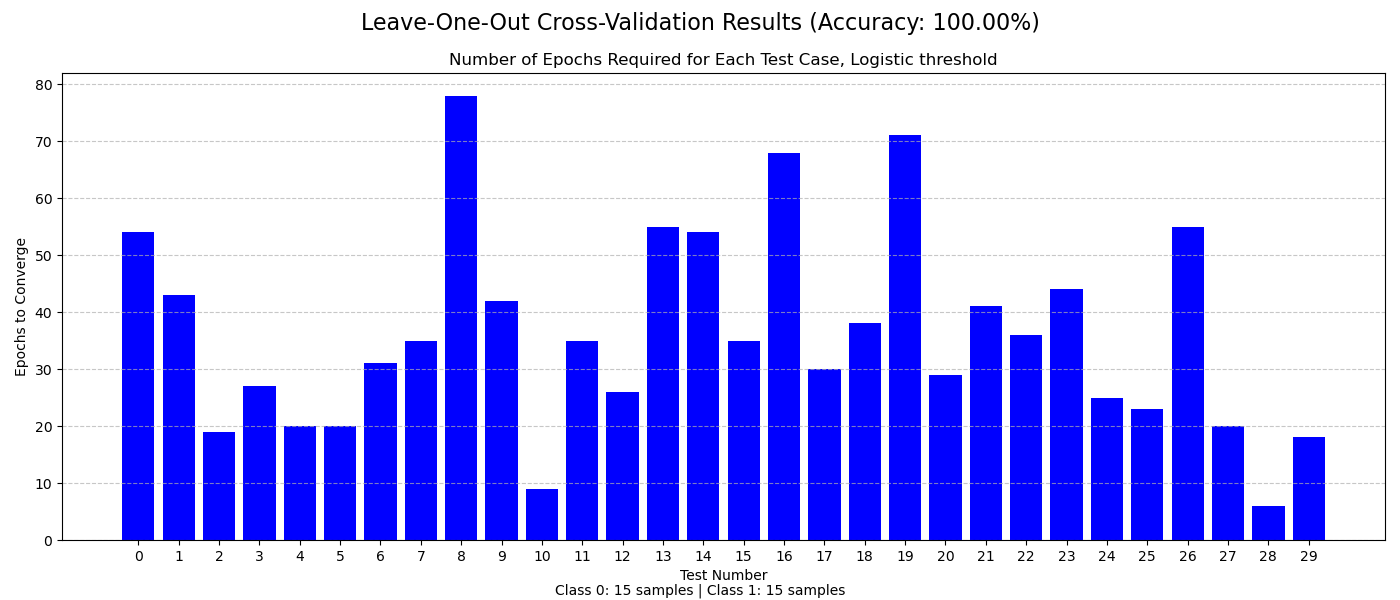
\includegraphics[width=0.8\textwidth]{figures/classifier result 2.png}
    \caption{Leave-one-out cross-validation of the perceptron algorithm with hard threshold (top) and logistic function (bottom).}
    \label{fig:classifier_result}
\end{figure}


\begin{figure}
    \centering
    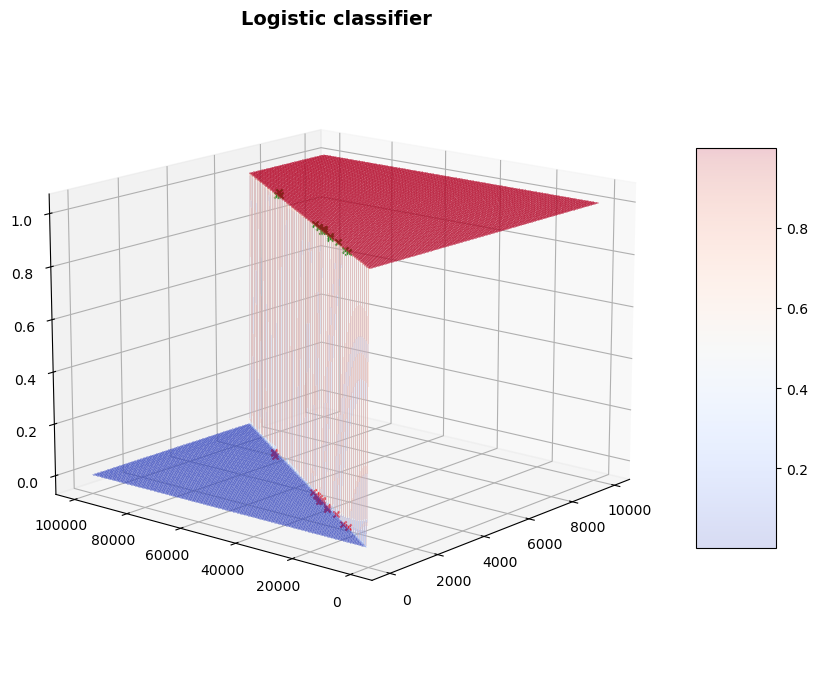
\includegraphics[width=0.8\textwidth]{figures/logistic classifier.png}
    \caption{Screenshot of the Jupyter notebook with the implementation of the perceptron algorithm.}
    \label{fig:logistic_classifier}
\end{figure}

We could not, or at least not without confusing tweaking of parameters, get a gradient descent algorithm to converge to a solution. The stochastic descent algorithm described above, however, worked. The convergence criteria we used was the average of the gradient every epoch.

\subsection{Experimenting with popular tools: \texttt{Keras}, \texttt{PyTorch}, \texttt{scikit\_learn}}

\subsection{Reading Ruder}
You will read the article An overview of gradient descent optimization algorithms by Ruder (2017) and you will outline the main characteristics of all the optimization algorithms the author describes. This part should be of about one to two pages. 
\cite{DBLP:journals/corr/Ruder16}


\section{Conclusions and future work}


\printbibliography
\end{document}